\documentclass[11pt,a4paper]{article}
\usepackage{fontspec}
\setmainfont{FreeSerif.otf}[
 BoldFont=FreeSerifBold.otf, ItalicFont=FreeSerifItalic.otf,
 BoldItalicFont=FreeSerifBoldItalic.otf]
\setsansfont{FreeSans.otf}[
 BoldFont=FreeSansBold.otf, ItalicFont=FreeSansOblique.otf]
\setmonofont{FreeMono.otf}
\usepackage[russian,english]{babel}
\usepackage[margin=25mm]{geometry}
\usepackage{amsmath,amssymb,amsthm,mathtools}
\usepackage{booktabs,tabularx,graphicx,microtype}
\newcolumntype{Y}{>{\raggedright\arraybackslash}X}
\setlength{\emergencystretch}{1em}
\usepackage[numbers,sort&compress]{natbib}
\usepackage{xcolor}
\definecolor{linkblue}{HTML}{254B79}
\usepackage[colorlinks=true,allcolors=linkblue]{hyperref}
\usepackage{enumitem}
\setlist{itemsep=3pt,topsep=5pt}
\newtheorem{theorem}{Теорема}
\newtheorem{lemma}[theorem]{Лемма}
\newtheorem{proposition}[theorem]{Утверждение}
\newtheorem{corollary}[theorem]{Следствие}
\theoremstyle{definition}
\newtheorem{definition}[theorem]{Определение}
\theoremstyle{remark}
\newtheorem{remark}[theorem]{Замечание}
\addto\captionsrussian{\renewcommand{\proofname}{Доказательство}}
\newcommand{\KL}{\operatorname{KL}}
\newcommand{\E}{\mathbb E}
\renewcommand{\Prob}{\mathbb P}
\newcommand{\Bern}{\operatorname{Bern}}
\newcommand{\Beta}{\operatorname{Beta}}
\newcommand{\Geom}{\operatorname{Geom}}
\newcommand{\Var}{\operatorname{Var}}
\newcommand{\bits}{\mathrm{bit}}
\DeclareMathOperator*{\argmin}{arg\,min}
\DeclareMathOperator*{\argmax}{arg\,max}
\hypersetup{pdftitle={Асимптотика requential-кодирования и восстановление конечной модели},
 pdfauthor={Алябушев, Дементьев, Курдюков, Чирков}}
\title{Асимптотика requential-кодирования\\и восстановление конечной модели}
\author{Алябушев \and Дементьев \and Курдюков \and Чирков}
\date{23 ноября 2026 г.}
\begin{document}
\selectlanguage{russian}
\maketitle
\begin{abstract}
Длины кодов данных, траекторий обучения и конечных предикторов характеризуют
разные объекты. Мы исследуем, как протокол передачи влияет на измеряемую
сложность. Для детерминированного бернуллиевского учителя и ученика с априорным
распределением $\Beta(a,b)$ доказывается оценка оптимальной ожидаемой длины
requential-записи $A(a)\ln(1/\varepsilon)+O(1)$ при конечном KL-риске не выше
$\varepsilon$. Коэффициент определяется одномерной оптимизацией, а геометрические
расписания пакетов достигают его. Получена также точная ведущая константа при
ограничении среднего числа кандидатов на пакет. Замена замороженного предиктора
совместным байесовским предиктивом уменьшает оптимальную ведущую константу до
$a/\ln 2$. Для факторизованной линейной регрессии выведена классификация
накопленного риска при убывающем шаге: предельный дисбаланс факторов задаёт
степенной показатель, а при точном балансе сумма растёт как $T/\ln^2 T$.
Наконец, для сжимающего отображения обновления построено описание конечного
состояния ожидаемой длины $O(\ln(1/\delta))$, не зависящей от горизонта обучения.
Доказательства и воспроизводимые аналитические примеры показывают, какие
различия между оценками сложности вызваны геометрией модели, а какие ---
алгоритмом обучения и правилами кодирования.
\end{abstract}
\noindent\textbf{Ключевые слова:} минимальная длина описания; requential-кодирование;
байесовский предиктив; расписание пакетов; факторизованная регрессия;
сжатие траектории.

\section{Введение}

Число параметров описывает размер представления нейросети, но само по себе не
определяет стоимость передачи её предсказаний или качество обобщения. Один и тот
же предиктор можно представить разными наборами весов; одна архитектура при
разных данных и правилах обучения даёт разные результаты. Принцип минимальной
длины описания (minimum description length, MDL) предлагает выбирать модель
вместе с кодом, который объясняет наблюдения коротким сообщением
\citep{grunwald2004}. Для нейросетей этот подход реализуется через вариационное
кодирование, приближения маргинального правдоподобия, последовательные коды и
компрессию весов \citep{graves2011,ritter2018,blier2018,arora2018}.

Однако даже длина в битах не является универсальной характеристикой модели:
результат зависит от того, \emph{что} восстанавливает получатель. В
prequential-кодировании передаются наблюдения, и декодер обучается на уже
раскрытом префиксе \citep{blier2018,bornschein2022}. В requential-кодировании
передаются индексы примеров, сгенерированных из распределения ученика и
выбранных учителем \citep{finzi2026,qiu2026}. В коде весов передаётся конечное
состояние модели. Обучающие последовательности с совершенно разными длинами
могут приводить к близким конечным состояниям. Поэтому сравнение этих величин
требует явного задания протокола.

Мы исследуем асимптотику стоимости requential-кодирования при заданной
точности конечного предиктора. Рассматриваются три вопроса. Как выбирать моменты
обновления ученика, если каждый переданный пакет имеет собственные накладные
расходы? Определяется ли накопленный риск геометрическим коэффициентом
байесовского обучения, когда вместо интегрирования по параметрам используется
градиентный спуск? И когда полную запись обучения можно заменить коротким
описанием его конечного результата?

Мы получаем следующие результаты.
\begin{enumerate}
\item Для замороженного внутри пакета предиктора с априорным распределением
$\Beta(a,b)$ и нулевого
учителя доказываем
\[
 C_{\rm fr}(\varepsilon)=A(a)\ln(1/\varepsilon)+O(1),\qquad
 A(a)=\min_{r>1}\frac{L(a(r-1))}{\ln r},
\]
где $L(h)$ --- ожидаемая длина $\delta$-кода Элиаса для геометрического индекса
со средним $e^h$. Параметр $b$ влияет на конечные поправки, но не на ведущий
коэффициент. При ограничении среднего числа кандидатов область минимизации
по $r$ сужается явным образом.
\item Показываем, что совместное байесовское предсказание пакета меняет ведущий
коэффициент на $a/\ln 2<A(a)$. Таким образом, при фиксированных априорном
распределении, учителе и конечном риске стоимость зависит от способа
формирования пакета.
\item Для точного градиентного спуска в факторизованной регрессии с нулевой
истинной матрицей доказываем степенной закон, зависящий от предельного
дисбаланса норм. Дополняем его случаем точного баланса:
$K_t\sim(8\gamma^2\ln^2t)^{-1}$ при шаге $\gamma/(t+t_0)$.
\item Для сжимающих обновлений строим requential-описание конечной точки по
короткому суффиксу меток. Его ожидаемая длина ограничена через точность
восстановления и не растёт с длиной исходной траектории.
\end{enumerate}

Эти результаты относятся к явно заданным классам кодов и алгоритмов. В
частности, нижняя оценка для протокола с обязательным индексом на пакет не
является нижней оценкой колмогоровской сложности конечной модели. Аналитические
примеры ниже служат проверкой формул; перенос выводов на большие нейросети
требует отдельных экспериментов.

\section{Кодируемый объект и постановка задачи}
\label{sec:setup}

\subsection{Разные значения длины описания}

Пусть наблюдения $Y_1,Y_2,\dots$ независимы и имеют распределение $Q$,
а $P_n$ --- предиктор после $n$ обучающих примеров.
Все дивергенции и натуральные логарифмы измеряются в натах;
$\log_2$ и длины бинарных сообщений --- в битах. Положим
\[
 K_n=\KL(Q\Vert P_n),\qquad S(N)=\sum_{n=0}^{N-1}K_n.
\]
Для случайной истории $K_n$ также случайна.

Если байесовский предиктор обновляется после каждого наблюдения, то цепное
правило даёт точное равенство
\begin{equation}
 \E[-\ln P(Y_{1:N})]=NH(Q)+\sum_{n=0}^{N-1}\E K_n.
 \label{eq:prequential}
\end{equation}
Здесь $H(Q)$ --- энтропия одного дискретного наблюдения в натах, а
$P(Y_{1:N})$ --- байесовская смесь. Избыточность правой части не следует
отождествлять с длиной отдельного сообщения о весах.

В регулярных моделях при стандартных условиях ведущий коэффициент байесовской
избыточности равен половине размерности. Для параметрического семейства
$p_\theta$ с априорной мерой $\Pi$ определим эмпирическую потерю и байесовскую
свободную энергию:
\[
 L_N(\theta)=-\frac1N\sum_{i=1}^{N}\ln p_\theta(Y_i),\qquad
 F_N=-\ln\int e^{-NL_N(\theta)}\,\Pi(d\theta).
\]
Пусть $Q$ реализуется параметром $\theta_*$ этого семейства. В сингулярной
модели при условиях аналитичности и интегрируемости сингулярной теории обучения
в разложении $F_N$ появляются действительный лог-канонический порог (RLCT)
$\lambda$ и кратность $m$ \citep{watanabe2009,watanabe2013}:
\begin{equation}
 F_N=NL_N(\theta_*)
       +\lambda\ln N-(m-1)\ln\ln N+O_{\Prob}(1).
 \label{eq:slt}
\end{equation}
Здесь $O_{\Prob}(1)$ обозначает ограниченный по вероятности остаток.
Это разложение характеризует байесовское интегрирование по параметрам;
асимптотика отдельной оптимизационной траектории требует самостоятельного
анализа. Связь RLCT с практической сжимаемостью исследуется, в частности,
в \citet{urdshals2025}.

\subsection{Requential-протокол}

На каждом шаге кодер и декодер знают состояние ученика, правило обновления и
размер следующего пакета $B$. Кодер использует учителя $Q$ для выбора пакета
из общего потока кандидатов; декодеру достаточно полученного индекса.
В основе выбора лежит пуассоновское функциональное представление (PFR)
\citep{li2018}. Для распределения предложения $P$ и $Q\ll P$ положим
$R=dQ/dP$. Пусть $T_1<T_2<\dots$ --- времена прихода пуассоновского процесса
единичной интенсивности, а $X_1,X_2,\dots$ --- независимые метки с законом $P$,
не зависящие от времён. Тогда
\[
 J=\argmin_{j\ge1}\frac{T_j}{R(X_j)},\qquad X_J\sim Q,
\]
где при $R(X_j)=0$ отношение принимается равным $+\infty$.
Процесс времён и меток составляет общую случайность кодера и декодера;
для разных пакетов используются её независимые части.

В основном протоколе распределение предложения для пакета равно
$P_n^{\otimes B}$: состояние ученика заморожено до конца пакета. Распределение
выбранного пакета равно $Q^{\otimes B}$. Индекс $J\ge1$ передаётся отдельным
$\delta$-кодом Элиаса \citep{elias1975}, имеющим длину
\begin{equation}
 \ell_\delta(j)=\lfloor\log_2j\rfloor
  +2\left\lfloor\log_2(\lfloor\log_2j\rfloor+1)\right\rfloor+1.
 \label{eq:elias}
\end{equation}
В частности, $\ell_\delta(1)=1$: даже совпадение распределений не устраняет
обязательное сообщение. Для пакетной дивергенции $h=BK_n$ используется
известная условная верхняя оценка \citep[приложение A]{qiu2026}
\begin{equation}
 \E[\ell_\delta(J)\mid\text{история}]
 \le f(h/\ln2),\qquad
 f(d)=d+2\log_2(1+d)+\kappa,
 \quad 0<\kappa<5.21.
 \label{eq:universal-bound}
\end{equation}
Здесь используется константа
$\kappa=1+\beta+2\log_2(1+\beta)$ при $\beta=1+(e\ln2)^{-1}$.
Правая часть оценивает условное математическое ожидание длины сообщения.

Фиксируем заранее детерминированное расписание
$0=n_0<n_1<\dots<n_m=N$, $B_i=n_{i+1}-n_i$.
Правило остановки, $N$, априорное распределение, правило обновления и код
известны обеим сторонам;
их описание в рассматриваемую условную длину не входит. Расписание,
подобранное после наблюдения неизвестных декодеру данных, требует отдельной
передачи. В разделе~\ref{sec:batch} учитель детерминирован, поэтому все
состояния и оптимальные расписания вычисляются по публичным параметрам.

\subsection{Отличие от существующих постановок}

Работы о prequential-кодах исследуют последовательное обучение, replay и
калибровку \citep{blier2018,bornschein2022}. В \citet{finzi2026} requential-код
вводится как способ описать усвоенную структуру. В \citet{qiu2026} развито
сжатие модели через выбранные данные; в формуле (21) рассматривается разбиение
\emph{уже заданного} обучающего пакета на сообщения при сохранении исходных
обновлений. Здесь размер пакета определяет следующее обновление ученика и
потому меняет его будущие предсказания. Наша оптимизация проводится при
фиксированном конечном риске.

Анализ линейных факторизаций связан с работами об инвариантах баланса и
неявном смещении градиентного потока \citep{du2018,tarmoun2021,min2022}.
Мы рассматриваем дискретный спуск с гармонически убывающим шагом и вычисляем
асимптотику \emph{суммы} рисков. Восстановление конечной точки связано с
последовательным обучением управляемым учителем \citep{lessard2019}; цена
управляющего действия у нас задаётся длиной индекса в общем потоке.

\section{Оптимальное расписание пакетов}
\label{sec:batch}

\subsection{Точная стоимость для нулевого учителя}

Пусть $Q=\Bern(0)$, а априорное распределение вероятности единицы равно
$\Beta(a,b)$, где $a,b>0$. После $n$ нулей апостериорное распределение имеет вид
$\Beta(a,b+n)$. Одношаговый байесовский предиктор и его риск равны
\begin{equation}
 P_n(1)=\frac{a}{n+a+b},\qquad
 P_n(0)=\frac{n+b}{n+a+b},\qquad
 K_n=\ln\left(1+\frac{a}{n+b}\right).
 \label{eq:beta-risk}
\end{equation}
Следовательно, минимальный объём для риска не выше $\varepsilon$ равен
\begin{equation}
 N_\varepsilon=\max\left\{0,
  \left\lceil\frac{a}{e^\varepsilon-1}-b\right\rceil\right\}
   \sim\frac{a}{\varepsilon}.
 \label{eq:target-N}
\end{equation}

Учитель выбирает только полностью нулевой пакет. В PFR минимум среди таких
кандидатов достигается на первом из них: их отношения плотностей одинаковы,
а времена прихода строго возрастают. При замороженном предикторе вероятность
успеха одного кандидата равна $P_n(0)^B=e^{-BK_n}$. Поэтому
\begin{equation}
 J\sim\Geom(e^{-h}),\quad h=BK_n,\qquad
 c_{\rm fr}(n,B)=L(BK_n),\quad
 L(h)=\E_{J\sim\Geom(e^{-h})}\ell_\delta(J).
 \label{eq:exact-transition}
\end{equation}
Здесь геометрическое распределение имеет носитель $\{1,2,\dots\}$, так что
$\E J=e^h$. В данной специальной модели индекс можно найти простым поиском
первого успеха; общий PFR-поиск сложнее.

\begin{lemma}[Средняя длина геометрического индекса]
\label{lem:length}
Функция $L$ непрерывна на $[0,\infty)$, не убывает, $L(0)=1$ и является
непрерывно дифференцируемой на $(0,\infty)$. Для $h\ge0$
\begin{equation}
 L(h)=1+\sum_{j=1}^{\infty}d_j(1-e^{-h})^{2^j-1},\qquad
 d_j=\begin{cases}3,&j+1\text{ --- степень двойки},\\1,&\text{иначе}.
 \end{cases}
 \label{eq:dyadic-series}
\end{equation}
Кроме того,
\begin{equation}
 L(h)\ge\max\{1,h/\ln2\},\qquad
 L(h)\le\frac{h}{\ln2}
      +2\log_2\left(1+\frac{h}{\ln2}\right)+1.
 \label{eq:L-bounds}
\end{equation}
\end{lemma}
\begin{proof}
Длина~\eqref{eq:elias} меняется только при переходе индекса через $2^j$.
Приращение равно $d_j$. Формула ожидания через вероятности превышения порогов
даёт~\eqref{eq:dyadic-series}. На каждом отрезке $0\le h\le H<\infty$ ряд
равномерно сходится, поскольку его члены ограничены величинами
$3(1-e^{-H})^{2^j-1}$. На компактных подотрезках $(0,\infty)$ так же сходится
ряд производных. Монотонность следует из монотонности каждого слагаемого.

Нижняя граница единицей очевидна. Для $h>0$ вероятность любого значения
геометрического индекса не выше $e^{-h}$, поэтому его энтропия не меньше
$h/\ln2$. Средняя длина префиксного кода не меньше энтропии. Для верхней
границы используем
$\ell_\delta(j)\le\log_2j+2\log_2(1+\log_2j)+1$ и дважды неравенство Йенсена:
$\E\log_2J\le\log_2\E J=h/\ln2$.
\end{proof}

Обозначим через $V_{a,b}(N)$ минимальную ожидаемую сумму длин отдельных индексов
среди публичных расписаний, заканчивающихся ровно на $N$. Через
$C_{\rm fr}(\varepsilon)$ обозначим минимум при условии
$K_N\le\varepsilon$. Расписания конечны; при $N=0$ сообщения не требуются.

\begin{theorem}[Ведущий коэффициент и ограниченный остаток]
\label{thm:optimal}
Для любых $a,b>0$ положительный конечный минимум
\begin{equation}
 A(a)=\min_{r>1}\frac{L(a(r-1))}{\ln r}
 \label{eq:A}
\end{equation}
достигается. При $N\to\infty$ и $\varepsilon\downarrow0$ справедливы
\begin{align}
 V_{a,b}(N)&=A(a)\ln(N+b)+O_{a,b}(1),
 \label{eq:finite-asymp}\\
 C_{\rm fr}(\varepsilon)&=A(a)\ln(1/\varepsilon)+O_{a,b}(1).
 \label{eq:eps-asymp}
\end{align}
Для каждого $N$ имеется явная нижняя оценка
\begin{equation}
 V_{a,b}(N)\ge
 A(a)\ln\frac{N+b+a}{b+a}.
 \label{eq:finite-lower}
\end{equation}
Геометрический рост $n+b$ с любым минимизатором $r_*$
в~\eqref{eq:A}, с целочисленным округлением и усечением последнего пакета,
достигает~\eqref{eq:finite-asymp}.
\end{theorem}
\begin{proof}
При $r\downarrow1$ отношение в~\eqref{eq:A} стремится к бесконечности, так как
$L\ge1$. При $r\to\infty$ оно не меньше
$a(r-1)/(\ln2\ln r)$ и также стремится к бесконечности. Непрерывность $L$
обеспечивает достижение положительного конечного минимума.

Из $\ln(1+x)\ge x/(1+x)$ и монотонности $L$ для любого перехода следует
\[
 L(BK_n)\ge L\left(\frac{aB}{n+b+a}\right)
 \ge A(a)\ln\left(1+\frac{B}{n+b+a}\right).
\]
Сумма логарифмов по расписанию телескопируется, что
даёт~\eqref{eq:finite-lower}.

Для верхней оценки зафиксируем минимизатор $r_*>1$ и положим на бесконечном
расписании
\[
 B(n)=\max\{1,\lfloor(r_*-1)(n+b)\rfloor\}.
\]
Пишем $x=n+b$. После конечного числа начальных шагов
\[
 B=(r_*-1)x+O(1),\quad
 \ln\frac{x+B}{x}=\ln r_*+O(x^{-1}),\quad
 B\ln(1+a/x)=a(r_*-1)+O(x^{-1}).
\]
Величина $x$ растёт геометрически, поэтому сумма $x^{-1}$ по шагам конечна.
Лемма~\ref{lem:length} даёт локальную липшицевость $L$ в окрестности
$a(r_*-1)>0$. После $m$ полных пакетов суммарная стоимость равна
$mL(a(r_*-1))+O(1)$, а прирост $\ln x$ --- $m\ln r_*+O(1)$.
Перед первым превышением $N$ укорачиваем последний пакет. Его стоимость
ограничена константой, как и отличие $\ln x$ от логарифма конечной точки
полного пакета. Получаем верхнюю оценку в~\eqref{eq:finite-asymp}.

Любое расписание до $N'>N$ можно усечь на $N$: последняя стоимость уменьшится
по монотонности $L$. Поэтому $V_{a,b}(N)$ не убывает и
$C_{\rm fr}(\varepsilon)=V_{a,b}(N_\varepsilon)$.
Подстановка~\eqref{eq:target-N} завершает доказательство.
\end{proof}

Параметр $a$ имеет также геометрическую интерпретацию. Если $p=w^k$ при
равномерном $w\in[0,1]$, то $p\sim\Beta(1/k,1)$ и $a=1/k$.
Для нулевого учителя $K(w)=-\ln(1-w^k)\sim w^k$, так что априорная масса
множества $\{K(w)<\varepsilon\}$ имеет порядок $\varepsilon^{1/k}$.
В этой граничной модели показатель априорной массы равен $a$.
Теорема~\ref{thm:optimal} устанавливает его связь с длиной записи через
точную формулу~\eqref{eq:beta-risk} и справедлива для любого вещественного
$a>0$.

\begin{proposition}[Конечный оптимум]
\label{prop:dp}
Минимальная длина до фиксированного $N$ вычисляется рекурсией
\begin{equation}
 V_{a,b}(0)=0,\qquad
 V_{a,b}(j)=\min_{0\le n<j}
 \left\{V_{a,b}(n)+L\left((j-n)\ln\left(1+\frac a{n+b}\right)\right)\right\}.
 \label{eq:dp}
\end{equation}
Она требует $O(N^2)$ вычислений стоимости перехода и $O(N)$ памяти для
значений и предшественников. Хранение всей матрицы стоимостей дополнительно
требует $O(N^2)$ памяти.
\end{proposition}
\begin{proof}
Последний переход оптимального пути в вершину $j$ начинается в некотором
$n<j$. Его предыстория также должна быть оптимальной, иначе её можно заменить
на более дешёвую. Обратное утверждение следует приписыванием последнего
перехода. Получается кратчайший путь в ациклическом графе объёмов выборки.
\end{proof}

\subsection{Ограничение числа кандидатов}

Оценка длины не учитывает стоимость поиска индекса. В нашей модели ожидаемое
число просмотренных кандидатов на шаге в точности равно $e^{BK_n}$.
Потребуем, чтобы оно не превышало публичную константу $M$ на каждом шаге.
Непустое расписание существует тогда и только тогда, когда
$M\ge1+a/b$: уже первый пакет содержит не менее одного наблюдения.

\begin{theorem}[Оптимум при ограничении поиска]
\label{thm:compute}
Пусть $M\ge1+a/b$. Для оптимальной ожидаемой длины среди расписаний с
$\E J_i\le M$ на каждом шаге справедливо
\begin{equation}
 C_{{\rm fr},M}(\varepsilon)
 =A_M(a)\ln(1/\varepsilon)+O_{a,b,M}(1),\qquad
 A_M(a)=\min_{1<r\le1+\ln M/a}
       \frac{L(a(r-1))}{\ln r}.
 \label{eq:compute-opt}
\end{equation}
Коэффициент $A_M(a)$ не возрастает по $M$. Если область минимизации содержит
хотя бы один минимизатор~\eqref{eq:A}, то $A_M(a)=A(a)$.
\end{theorem}
\begin{proof}
Для любого допустимого перехода
\[
 \frac{aB}{n+b+a}\le BK_n\le\ln M.
\]
Следовательно, $r=1+B/(n+b+a)$ принадлежит области в~\eqref{eq:compute-opt}.
Нижняя оценка из доказательства теоремы~\ref{thm:optimal} сохраняется с $A_M$.

Для верхней оценки выбираем минимизатор $r_M$ и $h_*=a(r_M-1)\le\ln M$.
Используем правило
\[
 B(n)=\max\{1,\lfloor h_*/K_n\rfloor\}.
\]
Если округление даёт ноль, пакет из одного наблюдения допустим, поскольку
$K_n\le K_0\le\ln M$. После конечного начального участка
$BK_n=h_*+O((n+b)^{-1})$ и
$B/(n+b)=h_*/a+O((n+b)^{-1})$.
Поэтому стоимость и логарифмический прирост имеют те же суммируемые остатки,
что и в предыдущем доказательстве. Последний пакет можно укоротить без
нарушения ограничения. Монотонность $A_M$ следует из вложенности областей.
\end{proof}

При таком расписании число сообщений имеет порядок $\ln(1/\varepsilon)$.
Такой же порядок имеет ожидаемое суммарное число просмотренных пакетов
из потока кандидатов.
Если генерация одного пакета из $B$ наблюдений стоит $O(B)$, суммарная
ожидаемая стоимость их генерации равна $O(N_\varepsilon)=O(1/\varepsilon)$:
$\sum_i B_i\E J_i\le MN_\varepsilon$. Это утверждение относится к генерации
кандидатов; стоимость обучения модели учитывается отдельно.

\subsection{Совместный предиктив вместо замороженного}

У байесовского ученика имеется другой естественный способ генерировать пакет:
выбрать параметр из апостериорного распределения и затем получить $B$
условно независимых меток.
Такое распределение совпадает с последовательным предсказанием с
внутрипакетным обновлением. Оно отличается от $P_n^{\otimes B}$.
Для полностью нулевого пакета его вероятность равна
\begin{equation}
 P_n^{\rm joint}(0^B)=\frac{\mathrm B(a,b+n+B)}{\mathrm B(a,b+n)},\qquad
 h_{\rm joint}(n,B)=\ln\frac{\mathrm B(a,b+n)}{\mathrm B(a,b+n+B)},
 \label{eq:joint}
\end{equation}
где $\mathrm B$ --- бета-функция. Индекс первого нулевого кандидата по-прежнему
геометрический, а его стоимость равна $L(h_{\rm joint}(n,B))$.
Конечное апостериорное распределение после $N$ нулей то же, что у замороженного
протокола.

\begin{theorem}[Зависимость ведущей константы от предиктива]
\label{thm:joint}
Обозначим через $C_{\rm joint}(\varepsilon)$ оптимальную ожидаемую длину
записи с предложением~\eqref{eq:joint}, теми же априорным распределением,
кодом индекса и условием
конечного риска. При $\varepsilon\downarrow0$
\begin{equation}
 C_{\rm joint}(\varepsilon)=\frac a{\ln2}\ln(1/\varepsilon)
                  +O(\ln\ln(1/\varepsilon)),
 \qquad \frac a{\ln2}<A(a).
 \label{eq:joint-asymp}
\end{equation}
Один пакет из $N_\varepsilon$ наблюдений уже достигает этой ведущей константы.
\end{theorem}
\begin{proof}
Для любого расписания приращения~\eqref{eq:joint} телескопируются:
\[
 \sum_i h_{\rm joint}(n_i,B_i)=
 H_N:=\ln\frac{\mathrm B(a,b)}{\mathrm B(a,b+N)}
      =a\ln N+O_{a,b}(1).
\]
Последнее равенство следует из
$\Gamma(N+a+b)/\Gamma(N+b)\sim N^a$.
По~\eqref{eq:L-bounds} стоимость любого расписания не меньше $H_N/\ln2$.
Для одного пакета её значение равно $L(H_N)$ и не превосходит
$H_N/\ln2+2\log_2(1+H_N/\ln2)+1$.
Поскольку $H_N$ возрастает, условие $N\ge N_\varepsilon$ и
\eqref{eq:target-N} дают требуемую асимптотику.

Для замороженного протокола минимум достигается в конечной точке $r_*>1$.
Используя $L(h)\ge h/\ln2$ и $r_*-1>\ln r_*$, получаем
\[
 A(a)\ge\frac{a(r_*-1)}{\ln2\ln r_*}>\frac a{\ln2}.
\]
\end{proof}

Выигрыш в длине сопровождается ростом поиска: у одного совместного пакета
$\E J=e^{H_N}=\Theta(N^a)$, тогда как геометрическое расписание замороженных
пакетов удерживает эту величину ограниченной. Теорема~\ref{thm:joint}
не утверждает оптимальность одного пакета по времени.

\begin{remark}[Область нижних оценок]
Нулевой учитель выбран для точного анализа. Если декодеру разрешено пропустить
индексы и просто получить $N$ нулей, он воспроизведёт апостериорное распределение без сообщения
при публичном $N$. Поэтому положительные константы выше характеризуют класс
протоколов с \emph{обязательной отдельной передачей индекса каждого пакета}.
Они не являются нижними границами для всех способов передачи этой модели.
\end{remark}

\subsection{Случайный учитель и ожидаемая верхняя оценка}

Для $Q=\Bern(q)$, $0<q<1$, состояние после $n$ выбранных примеров определяется
числом единиц $S_n\sim\operatorname{Bin}(n,q)$. Условно на $S_n=s$
вероятность единицы ученика равна $p=(s+a)/(n+a+b)$.
Для фиксированного публичного расписания стоимость перехода усредняется по
этому биномиальному распределению; размеры пакетов фиксируются независимо
от реализованных значений $s$.

Для распределений пакетов $P,Q$ положим $R(x)=Q(x)/P(x)$. Используя известный
условный закон PFR-индекса \citep[формулы (34)--(38)]{qiu2026}, получаем
\begin{equation}
 J\mid X=x\sim\Geom(M(x)^{-1}),\qquad
 M(x)=1+\sum_y P(y)(R(x)-R(y))_+.
 \label{eq:conditional-index}
\end{equation}
Отсюда точная ожидаемая стоимость равна
$\E_{S_n}\E_{X\sim Q^{\otimes B}}L(\ln M(X))$.
В бернуллиевской модели внутренняя сумма сводится к числу единиц в пакете,
так что все ожидания являются конечными биномиальными суммами. Рекурсия
\eqref{eq:dp} с этой усреднённой стоимостью находит оптимальное публичное
расписание до фиксированного $N$.

\begin{proposition}[Логарифмический порядок для суррогатной стоимости]
\label{prop:surrogate}
Пусть при любом детерминированном расписании распределение ученика после $n$
примеров одинаково, $K_n\ge0$, и для некоторых $0<c_1\le c_2<\infty$
\[
 \frac{c_1}{n+1}\le\E K_n\le\frac{c_2}{n+1}\quad(n\ge0).
\]
Минимальная сумма \emph{верхних оценок}
$\sum_i\E f(B_iK_{n_i}/\ln2)$ при $\E K_N\le\varepsilon$ имеет порядок
$\Theta(\ln(1/\varepsilon))$.
\end{proposition}
\begin{proof}
Так как $f(d)\ge d$, стоимость не меньше
\[
 \frac{c_1}{\ln2}\sum_i\frac{B_i}{n_i+1}
 \ge\frac{c_1}{\ln2}\ln(N+1).
\]
Условие риска требует $N+1\ge c_1/\varepsilon$. Для верхней оценки выбираем
удвоения $n+1$ и конечный объём порядка $c_2/\varepsilon$.
Тогда $B_i\E K_{n_i}$ ограничены, а число пакетов логарифмическое.
Вогнутость $f$ и неравенство Йенсена ограничивают каждый член сверху
константой.
\end{proof}

Доказательство не даёт нижнюю оценку фактической PFR-длины: из нижней
границы на верхнюю оценку нельзя вывести нижнюю границу на исходную величину.
Для шумного учителя точная асимптотическая константа оптимальной длины здесь
не установлена. На конечном горизонте точная стоимость и
\eqref{eq:universal-bound} могут выбирать разные расписания
(раздел~\ref{sec:validation}).

\section{Геометрический коэффициент и динамика обучения}
\label{sec:dynamics}

\subsection{Скалярный стохастический градиентный спуск}

Рассмотрим модель $Y=w_*X+\xi$, где $X\in\{-1,1\}$ равновероятен,
$\xi\sim\mathcal N(0,1)$, $X$ и $\xi$ независимы и наблюдения получаются
независимо. Ученик предсказывает
$\mathcal N(w_tX,1)$, поэтому условный популяционный KL-риск равен
$K_t=(w_t-w_*)^2/2$. Стохастический градиентный спуск (SGD) с функцией
потерь $\ell(w;X,Y)=(Y-wX)^2/2$ и усреднением градиента по пакету размера $B$
имеет вид
\[
 e_{t+1}=(1-\eta_t)e_t+\eta_t\zeta_t,\qquad
 e_t=w_t-w_*,\quad\E\zeta_t=0,\quad\E\zeta_t^2=B^{-1},
\]
где $\zeta_t$ независима от прошлого.

\begin{proposition}[Накопленный риск скалярного SGD]
\label{prop:scalar}
Если $0<\eta<2$ постоянно и начальная ошибка имеет конечный второй момент, то
\begin{equation}
 \E K_t\longrightarrow\frac{\eta}{2B(2-\eta)},\qquad
 \E\sum_{t<T}K_t=\frac{\eta}{2B(2-\eta)}T+O(1).
 \label{eq:constant-sgd}
\end{equation}
Если $\eta_t=\gamma/(t+t_0)$, $t_0>\gamma>1/2$, то
\begin{equation}
 \E K_t\sim\frac{\gamma^2}{2B(2\gamma-1)t},\qquad
 \E\sum_{t<T}K_t\sim\frac{\gamma^2}{2B(2\gamma-1)}\ln T.
 \label{eq:decaying-sgd}
\end{equation}
\end{proposition}
\begin{proof}
Для $v_t=\E e_t^2$ точно выполняется
\begin{equation}
 v_{t+1}=(1-\eta_t)^2v_t+\eta_t^2/B.
 \label{eq:variance-recurrence}
\end{equation}
При постоянном шаге стационарное значение равно
$v_*=\eta/[B(2-\eta)]$, а разность $v_t-v_*$ убывает геометрически.

Для убывающего шага положим $x=t+t_0$ и
$c=\gamma^2/[B(2\gamma-1)]$. Подстановка $v_t=c/x+z_t$
в~\eqref{eq:variance-recurrence} даёт
\[
 z_{t+1}=(1-\gamma/x)^2z_t+O(x^{-3}).
\]
Произведение множителей от $s$ до $t$ ограничено константой, умноженной на
$((s+t_0)/(t+t_0))^{2\gamma}$. Вариация постоянной даёт
$z_t=O(x^{-\min\{2\gamma,2\}}(1+\ln x))=o(x^{-1})$.
Отсюда $v_t\sim c/t$. Деление на два и суммирование завершают доказательство.
\end{proof}

Даже в регулярной скалярной модели накопление риска меняется с шагом и
размером пакета. При $\gamma=1$ и фиксированном $B$ пакетная дивергенция
$B\sum_{t<T}K_t$ имеет ведущий коэффициент $1/2$ при $\ln T$, но такое
совпадение не является универсальным тождеством для SGD.

\subsection{Нулевая факторизованная регрессия}

Пусть $u,v\in\mathbb R^2$, ученик предсказывает средний отклик $uv^\top x$,
истинный средний отклик равен нулю, шум гауссовский с единичной ковариацией,
а $\E XX^\top=I_2$. Тогда
\begin{equation}
 K(u,v)=\frac12\|uv^\top\|_F^2
       =\frac12\|u\|^2\|v\|^2.
 \label{eq:factor-risk}
\end{equation}
Точный градиентный спуск по популяционному риску даёт
\[
 u_{t+1}=(1-\eta_tb_t)u_t,\quad
 v_{t+1}=(1-\eta_ta_t)v_t,\quad
 a_t=\|u_t\|^2,\quad b_t=\|v_t\|^2.
\]
Следовательно,
\begin{align}
 a_{t+1}&=a_t(1-\eta_tb_t)^2,&
 b_{t+1}&=b_t(1-\eta_ta_t)^2,
 \label{eq:norm-recursion}\\
 a_{t+1}-b_{t+1}&=(a_t-b_t)(1-\eta_t^2a_tb_t).
 \label{eq:imbalance-recursion}
\end{align}
В непрерывном градиентном потоке разность квадратов норм сохраняется;
в дискретном спуске~\eqref{eq:imbalance-recursion} задаёт её изменение.

\begin{theorem}[Полная классификация при гармоническом шаге]
\label{thm:factorized}
Пусть $\eta_t=\gamma/(t+t_0)$, $\gamma>0$, $t_0>1$,
$a_0,b_0>0$ и $\gamma\max(a_0,b_0)<t_0$.
Положим $D_t=|a_t-b_t|$, $K_t=a_tb_t/2$ и $S(T)=\sum_{t<T}K_t$.

Если $D_0>0$, то $D_t\downarrow D_\infty>0$ и для некоторого $C>0$
\begin{equation}
 \alpha=2\gamma D_\infty,\qquad K_t\sim Ct^{-\alpha}.
 \label{eq:power-risk}
\end{equation}
Отсюда
\begin{equation}
 \begin{cases}
 S(T)\sim C T^{1-\alpha}/(1-\alpha),&0<\alpha<1,\\
 S(T)\sim C\ln T,&\alpha=1,\\
 S(\infty)-S(T)\sim C T^{1-\alpha}/(\alpha-1),&\alpha>1.
 \end{cases}
 \label{eq:sum-regimes}
\end{equation}
Предельный дисбаланс имеет вычислимый сертификат
\begin{equation}
 0\le D_t-D_\infty
 \le\frac{\gamma^2D_ta_tb_t}{t+t_0-1}.
 \label{eq:imbalance-certificate}
\end{equation}

Если $D_0=0$, то $a_t=b_t=s_t$ и
\begin{equation}
 s_t\sim\frac1{2\gamma\ln t},\qquad
 K_t\sim\frac1{8\gamma^2\ln^2t},\qquad
 S(T)\sim\frac{T}{8\gamma^2\ln^2T}.
 \label{eq:balanced}
\end{equation}
\end{theorem}
\begin{proof}
Начальное ограничение обеспечивает $0<\eta_ta_t,\eta_tb_t<1$.
Из~\eqref{eq:norm-recursion} по индукции следует, что $a_t,b_t$ положительны
и не возрастают. В~\eqref{eq:imbalance-recursion} множитель лежит в $(0,1)$,
так что знак $a_t-b_t$ сохраняется.

Пусть $a_0>b_0$. Поскольку $\sum_t\eta_t^2a_tb_t<\infty$ и все множители
строго положительны, произведение
\[
 D_t=D_0\prod_{s<t}(1-\eta_s^2a_sb_s)
\]
имеет положительный предел. В частности, $a_t\ge D_\infty$.
Из $1-x\le e^{-x}$ получаем
\[
 b_t\le b_0\exp\left(-2D_\infty\sum_{s<t}\eta_s\right)
       =O((t+t_0)^{-\alpha}),\qquad\alpha=2\gamma D_\infty>0.
\]
Таким образом, $b_t\to0$ и $a_t\to D_\infty$.

Оценим хвост произведения с помощью $1-\prod(1-x_s)\le\sum x_s$:
\[
 D_t-D_\infty
 \le D_t\sum_{s=t}^\infty\eta_s^2a_sb_s
 \le\gamma^2D_ta_tb_t\sum_{s=t}^\infty(s+t_0)^{-2}
 \le\frac{\gamma^2D_ta_tb_t}{t+t_0-1}.
\]
Это~\eqref{eq:imbalance-certificate}. В логарифме рекурсии для $b_t$
\[
 \ln b_{t+1}-\ln b_t
 =-2D_\infty\eta_t
   -2\eta_t\bigl(b_t+D_t-D_\infty\bigr)+O(\eta_t^2).
\]
Все остатки суммируемы: $\sum\eta_tb_t<\infty$ из степенной оценки,
$\sum\eta_t(D_t-D_\infty)<\infty$ из сертификата и
$\sum\eta_t^2<\infty$. Разность
$\sum_{s<t}\eta_s-\gamma\ln t$ имеет конечный предел. Поэтому
$\ln b_t+\alpha\ln t$ сходится к конечной константе, что даёт
$b_t\sim c t^{-\alpha}$ с $c>0$ и~\eqref{eq:power-risk}.
Случай $b_0>a_0$ симметричен. Суммирование эквивалентной степенной
последовательности доказывает~\eqref{eq:sum-regimes}.

Пусть теперь $a_0=b_0$. Баланс сохраняется, и
$s_{t+1}=s_t(1-\eta_ts_t)^2$. Для обратной нормы
\[
 \frac1{s_{t+1}}-\frac1{s_t}
 =\frac{2\eta_t-\eta_t^2s_t}{(1-\eta_ts_t)^2}
 =2\eta_t+O(\eta_t^2s_t).
\]
Остаток суммируем, поскольку $s_t\le s_0$ и
$\eta_ts_t\le\gamma s_0/t_0<1$. Следовательно,
$s_t^{-1}=2\gamma\ln t+O(1)$, откуда первые две
эквивалентности~\eqref{eq:balanced}. Последняя следует, например,
из теоремы Штольца для $\sum_{t<T}K_t$ и $T/\ln^2T$.
\end{proof}

Классификация относится к \emph{точному} популяционному градиенту. Для
стохастического градиента рекурсии~\eqref{eq:norm-recursion} содержат шум,
и перенос показателя $2\gamma D_\infty$ требует отдельной теоремы.

\subsection{Почему RLCT не определяет сумму рисков точного спуска}

В модели~\eqref{eq:factor-risk} можно явно вычислить показатель априорной
массы около множества нулевого риска.

\begin{proposition}[Одинаковая геометрия и разные скорости]
\label{prop:rlct-counterexample}
Пусть априорная мера на $(u,v)$ имеет ограниченную плотность с компактным носителем,
непрерывную и строго положительную в окрестности $(0,0)$.
Для $u,v\in\mathbb R^2$
\begin{equation}
 \Pi\{K(u,v)\le\varepsilon\}
  =\Theta(\varepsilon\ln(1/\varepsilon)),\qquad
 \int e^{-nK(u,v)}\,\Pi(du\,dv)=\Theta(n^{-1}\ln n).
 \label{eq:volume}
\end{equation}
Тем самым локальная геометрия имеет показатель $\lambda=1$ и логарифмическую
кратность $m=2$. Для одних и тех же риска и априорной меры существуют устойчивые
старты точного спуска, для которых $S(T)$ растёт быстрее $\ln T$, и другие
старты, для которых $S(T)$ сходится. Поэтому равенство
$S(T)\sim\lambda\ln T$ не является следствием одного лишь RLCT.
\end{proposition}
\begin{proof}
В полярных координатах в каждой из двух плоскостей мера с точностью до
угловой константы равна $da\,db$, где $a=\|u\|^2$, $b=\|v\|^2$.
В малом квадрате $0<a,b<c$ площадь области $ab\le2\varepsilon$ равна
\[
 \int_0^c\min\{c,2\varepsilon/a\}\,da
 =2\varepsilon\left(1+\ln\frac{c^2}{2\varepsilon}\right).
\]
Положительность плотности даёт нижнюю оценку, ограниченность плотности и
носителя --- верхнюю. Для интеграла используем интегрирование по функции
распределения риска $F(x)=\Pi(K\le x)$:
$\int e^{-nK}d\Pi=n\int_0^\infty e^{-nx}F(x)dx$.
Замена $z=nx$ и двусторонняя оценка на $F$ дают вторую формулу.

При точном балансе уже~\eqref{eq:balanced} даёт
$S(T)\asymp T/\ln^2T$. Для несбалансированного примера возьмём
$\gamma=1,t_0=10,a_0=0.2,b_0=0.05$:
$0<D_\infty<D_0=0.15$, так что $\alpha<0.3<1$.
Для $a_0=1,b_0=0.05$ сертификат уже при $t=0$ даёт
\[
 D_\infty\ge0.95-\frac{0.95\cdot1\cdot0.05}{9}>0.94,
\]
поэтому $\alpha>1$ и сумма сходится. Риск и априорная мера в этих примерах не меняются.
\end{proof}

Интерпретация~\eqref{eq:volume} как RLCT использует обычные условия
аналитической модели и гладкой положительной априорной плотности; сами двусторонние
оценки доказаны непосредственно. Различие скоростей показывает зависимость
оптимизационной записи от инициализации, сохраняя фиксированной геометрию
статистической модели.

\section{Описание конечного состояния}
\label{sec:endpoint}

\subsection{Восстановление по суффиксу}

Пусть состояние ученика принадлежит инвариантному множеству
$\mathcal S\subset\mathbb R^d$ и обновляется по метке из конечного алфавита
$\mathcal Y$:
$\theta_{t+1}=F_{Y_t}(\theta_t)$.
Декодер стартует из известного $\theta_0\in\mathcal S$. Требуется восстановить
предиктор $P_{\theta_T}$ с заданной ошибкой, а не обязательно повторить
все $T$ обновлений. Разрешены вспомогательные учителя, детерминированно
выбирающие нужную метку.

\begin{theorem}[Длина описания сжимающего ученика]
\label{thm:suffix}
Пусть для всех $y\in\mathcal Y$ и $\theta,\theta'\in\mathcal S$
\begin{align*}
 \|F_y(\theta)-F_y(\theta')\|&\le\rho\|\theta-\theta'\|,
                  &&0<\rho<1,\\
 \KL(P_\theta\Vert P_{\theta'})&\le C\|\theta-\theta'\|^2,
                  &&0<C<\infty,\\
 P_\theta(y)&\ge p_{\min}>0.
\end{align*}
Предположим также, что $\sup_{\theta\in\mathcal S}\|\theta-\theta_0\|\le R$
при некотором $R>0$.
Для $\delta>0$ положим
\begin{equation}
 h_\delta=\max\left\{0,
 \left\lceil\frac{\ln(CR^2/\delta)}{2\ln(1/\rho)}\right\rceil\right\},
 \qquad h=\min\{T,h_\delta\}.
 \label{eq:suffix-length}
\end{equation}
Повторение последних $h$ меток исходной траектории из $\theta_0$ даёт
состояние $\theta'$ с
$\KL(P_{\theta_T}\Vert P_{\theta'})\le\delta$.
Если для сокращённой записи используется заранее согласованный поток
кандидатов, независимый от исходной траектории, то существует сообщение
с ожидаемой длиной не выше
\begin{equation}
 \ell_\delta(h+1)+hL(-\ln p_{\min}).
 \label{eq:endpoint-code}
\end{equation}
В частности, равномерно по $T$ ожидаемая длина ограничена величиной
\begin{equation}
 \ell_\delta(h_\delta+1)+h_\delta L(-\ln p_{\min})
   =O(1+\ln(1/\delta)),\qquad \delta\downarrow0,
 \label{eq:endpoint-uniform}
\end{equation}
при фиксированных $C,R,\rho,p_{\min}$.
\end{theorem}
\begin{proof}
Если $T<h_\delta$, повторяем всю последовательность и получаем точное
состояние. Иначе истинное состояние перед суффиксом ---
$\theta_{T-h}$ --- удалено от $\theta_0$ не более чем на $R$.
Применение одной и той же последовательности из $h$ сжимающих отображений
даёт $\|\theta_T-\theta'\|\le R\rho^h$.
Тогда дивергенция не выше $CR^2\rho^{2h}\le\delta$.
Случай $h_\delta=0$ соответствует $CR^2\le\delta$.

Заголовок --- $\delta$-код числа $h+1$ --- сообщает декодеру количество
меток. Каждую нужную метку $y$ выбирает вспомогательный учитель с точечной
мерой $\delta_y$. Передаётся индекс её первого появления среди
независимых кандидатов из текущего предиктора. Для фиксированной исходной
траектории такой индекс имеет распределение
$\Geom(P_{\theta'}(y))$, и его ожидаемая стоимость не выше
$L(-\ln p_{\min})$. Независимость нового потока от исходной траектории
обеспечивает эту условную оценку даже при выборе суффикса по исходным данным.
После передачи каждой метки состояние воспроизводится точно. Складывая
стоимости, получаем~\eqref{eq:endpoint-code}.
Наконец, $h\le h_\delta$, функция $\ell_\delta$ не убывает,
$h_\delta=O(\ln(1/\delta))$, а длина заголовка имеет порядок
$O(1+\ln(h_\delta+1))$. Это доказывает~\eqref{eq:endpoint-uniform}.
\end{proof}

\begin{corollary}[Линейный разрыв с полной записью]
\label{cor:gap}
При условиях теоремы~\ref{thm:suffix} и фиксированной $\delta>0$ полная
requential-запись из $T$ единичных пакетов с отдельным индексом на шаг
имеет длину не менее $T$ битов. Минимальная ожидаемая стоимость описания
конечной точки ограничена константой, не зависящей от $T$.
\end{corollary}
\begin{proof}
Каждый индекс стоит хотя бы один бит. Верхняя оценка для конечной точки
дана~\eqref{eq:endpoint-code}.
\end{proof}

Это сравнение меняет цель декодирования: короткое сообщение восстанавливает
конечный предиктор с допуском, но не исходную случайную траекторию. Поэтому
разрыв не противоречит оптимальности исходного кода для более строгой задачи.
Предположение об инвариантности и сжатии существенно: для накопительного
среднего старые метки не теряют относительный вес экспоненциально, и
фиксированный суффикс обычно недостаточен.

\begin{corollary}[Аффинный бернуллиевский ученик]
\label{cor:affine}
Для обновления
\begin{equation}
 F_y(p)=\frac{p+1/8+3y/4}{2},\qquad
 p_0=\frac12,\qquad y\in\{0,1\},
 \label{eq:affine}
\end{equation}
отрезок $[1/8,7/8]$ инвариантен. Если $T\ge h$ и $p'$ восстановлено из
$p_0$ по последним $h$ меткам, то
\begin{equation}
 |p_T-p'|\le\frac38\,2^{-h},\qquad
 \KL(\Bern(p_T)\Vert\Bern(p'))\le\frac97\,4^{-h}.
 \label{eq:affine-bound}
\end{equation}
При $h=6$ дивергенция меньше $10^{-3}$ ната для любой исходной траектории.
\end{corollary}
\begin{proof}
Непосредственная проверка концов отрезка доказывает инвариантность.
Каждое обновление уменьшает разность состояний вдвое; начальное расхождение
между $p_{T-h}$ и $1/2$ не выше $3/8$.
Из $\ln x\le x-1$ следует
\[
 \KL(\Bern(p)\Vert\Bern(p'))
 \le\frac{(p-p')^2}{p'(1-p')}.
\]
Знаменатель не меньше $7/64$. Подстановка первой оценки
даёт~\eqref{eq:affine-bound}, причём $(9/7)4^{-6}<10^{-3}$.
\end{proof}

\subsection{Когда кодовая длина даёт гарантию обобщения}

Связь длины описания предиктора с риском на новых данных задаётся стандартной
границей для префиксного кода \citep{grunwald2004,arora2018}.

\begin{proposition}[Стандартная граница для кода предиктора]
\label{prop:occam}
Пусть $Z_1,\dots,Z_n$ независимы и одинаково распределены, убыток лежит в
$[0,1]$, а префиксный код и декодер $m\mapsto h_m$ фиксированы независимо от
выборки. Обозначим популяционный и эмпирический риски через
$R(h)=\E\mathcal L(h,Z)$ и
$\widehat R_n(h)=n^{-1}\sum_{i=1}^n\mathcal L(h,Z_i)$.
Для любого $\eta\in(0,1)$ с вероятностью не меньше $1-\eta$ одновременно для всех
сообщений $m$
\begin{equation}
 R(h_m)\le\widehat R_n(h_m)
 +\sqrt{\frac{\ell(m)\ln2+\ln(1/\eta)}{2n}}.
 \label{eq:occam}
\end{equation}
Если декодер использует общую случайность, она также должна быть независима
от выборки. В границу подставляется реализованная длина полного сообщения.
\end{proposition}
\begin{proof}
Условимся на общей случайности. Для каждого фиксированного сообщения
неравенство Хёффдинга ограничивает вероятность нарушения
\eqref{eq:occam} величиной $\eta2^{-\ell(m)}$.
По неравенству Крафта и объединению событий сумма этих вероятностей не
превосходит $\eta$. Остаётся усреднить по общей случайности.
\end{proof}

Сообщение $m$ может выбираться по данным, поскольку граница одновременна.
Длина $\ell(m)$ включает заголовок и все выбранные по данным параметры
декодирования. Граница относится к ограниченной функции потерь и к
декодированному предиктору $h_m$.

\section{Численные примеры}
\label{sec:validation}

\subsection{Граничная бернуллиевская модель}

Для расчёта ожидаемых длин используется ряд~\eqref{eq:dyadic-series}.
Математические ожидания для шумного учителя вычисляются полными
биномиальными суммами, а коэффициенты асимптотик --- одномерной
численной минимизацией.
Для ряда после $J$ порогов и $p=e^{-h}$ остаток ограничен величиной
\[
 3e^p\frac{e^{-p2^{J+1}}}{1-e^{-p2^{J+1}}}.
\]
Ряд обрывается при $p2^J\ge50$, что даёт остаток меньше $10^{-42}$;
суммы вычисляются в двойной точности. Минимумы локализуются на сетке и
уточняются ограниченной одномерной минимизацией.

\begin{table}[ht]
\centering
\caption{Численная оценка минимизатора замороженного протокола. Параметр $b$
не входит в ведущий коэффициент.}
\begin{tabular}{rrr}
\toprule
$a$ & $r_*$ & $A(a)$, бит/$\ln(1/\varepsilon)$\\
\midrule
0.10 & 5.780 & 1.252977\\
0.25 & 3.929 & 1.993603\\
0.50 & 2.922 & 2.976241\\
1.00 & 2.210 & 4.675413\\
\bottomrule
\end{tabular}

\label{tab:coef}
\end{table}

При $a=1/4$ получаем $r_*\approx3.928703$,
$h_*=a(r_*-1)\approx0.732176$ и $A(a)\approx1.993603$.
Ожидаемое число кандидатов в поздних пакетах приближается к
$e^{h_*}\approx2.079600$. Для $b=1$ ограничение $M=2$ немного повышает
ведущий коэффициент; при $M\ge2.079601$ этот численно найденный минимизатор
уже допустим. У совместного протокола ведущий коэффициент равен
$(1/4)/\ln2\approx0.360674$.

Для $N=63$, $a=1/4$, $b=1$ конечный риск всех сравниваемых расписаний равен
$\ln(1+0.25/64)\approx0.003899$ ната.

\begin{table}[ht]
\centering
\caption{Стоимость разных публичных расписаний при одинаковом конечном риске.}
\begin{tabular}{lrr}
\toprule
Размеры пакетов & Число сообщений & Ожидаемая длина, бит\\
\midrule
$3,12,48$ & 3 & 8.070631\\
$7,56$ & 2 & 9.303090\\
$63$ & 1 & 27.897764\\
63 пакета по одному & 63 & 66.297235\\
\bottomrule
\end{tabular}
\label{tab:N63}
\end{table}

Первое расписание --- оптимум рекурсии~\eqref{eq:dp}. Расписание $(7,56)$
минимизирует универсальную верхнюю оценку в этой задаче, но проигрывает
по фактическому математическому ожиданию. Таким образом, даже корректная
верхняя оценка может быть недостаточно точной для выбора протокола.

\begin{figure}[ht]
\centering
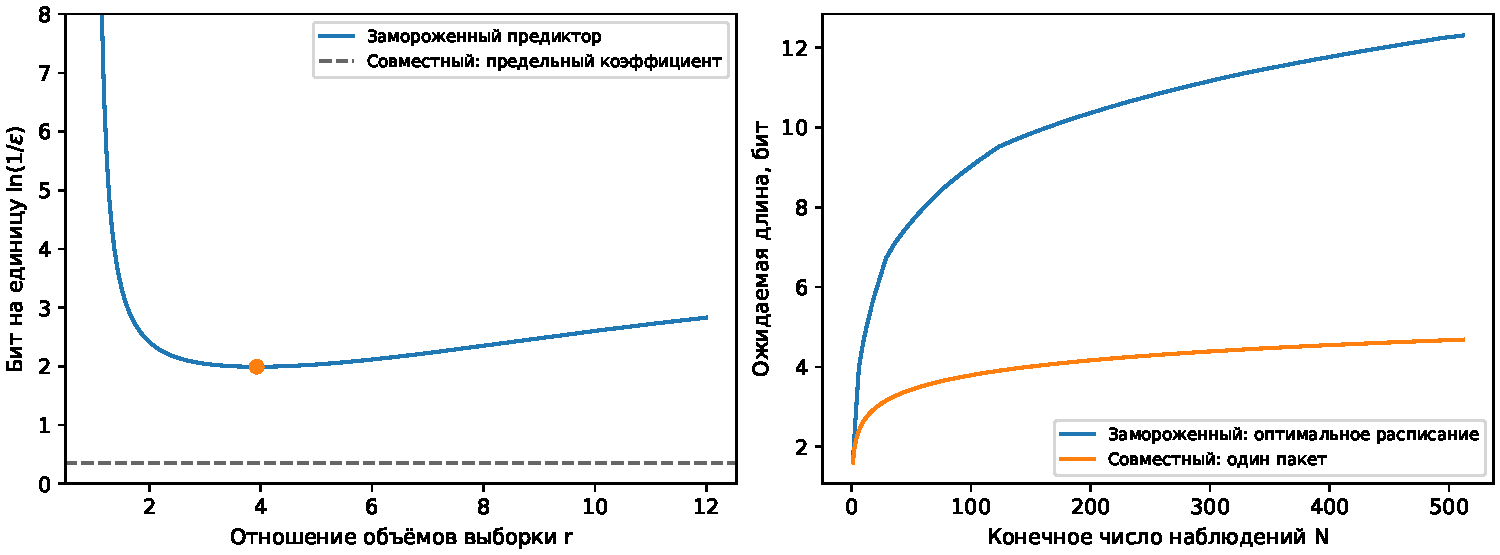
\includegraphics[width=\textwidth]{figures/protocol_costs.pdf}
\caption{Слева: ожидаемая стоимость замороженного пакета на единицу
логарифмического прироста объёма при $a=1/4$; пунктир --- ведущий коэффициент
совместного протокола. Справа: оптимальная конечная длина замороженного
протокола и стоимость одного совместного пакета при $b=1$.
Конечные длины совместного протокола могут быть заметно выше его ведущей
асимптотики из-за целочисленного кода индекса.}
\label{fig:protocol}
\end{figure}

Для оценки зависимости от второго параметра априорного распределения
на горизонте $N=256$
получены оптимальные длины $12.104019$, $10.839585$, $9.662267$ и $8.263138$
бита при $b=0.5,1,2,4$ соответственно. Это различие согласуется с тем, что
$b$ влияет на начальное состояние и ограниченный остаток, сохраняя $A(a)$,
как установлено в теореме~\ref{thm:optimal}.

\subsection{Шумный учитель}

При $q=0.20$, априорном распределении $\Beta(1,1)$ и $N=62$
ожидаемый конечный риск равен
приблизительно $0.007694$ ната. Точная
стоимость~\eqref{eq:conditional-index} и верхняя
оценка~\eqref{eq:universal-bound} выбирают разные расписания
(таблица~\ref{tab:noisy}). Оптимизация ожидаемой длины даёт экономию
$7.4715\%$. Результат относится к публичным детерминированным расписаниям
до $N=62$.

\begin{table}[ht]
\centering
\caption{Два критерия оптимизации. В обоих случаях конечный риск одинаков.}
\begin{tabular}{lrr}
\toprule
Размеры пакетов & Ожидаемая длина, бит & Сумма верхних оценок, бит\\
\midrule
$3,15,44$ & 10.255584 & 25.115133\\
$7,55$ & 11.083706 & 22.220445\\
\bottomrule
\end{tabular}
\label{tab:noisy}
\end{table}

\subsection{Проверка динамики и восстановления}

Для точного спуска при $\gamma=1,t_0=10$ и
$(a_0,b_0)=(0.2,0.05)$ расчёт до $T=2^{18}$ даёт
$D_T\approx0.149890564$. Оценка~\eqref{eq:imbalance-certificate}
ограничивает оставшееся уменьшение величиной $1.53\cdot10^{-10}$.
Соответствующий показатель $\alpha\approx0.299781128$ гарантированно меньше
единицы. Для старта $(1,0.05)$ получаем
$\alpha\approx1.896517056>1$. Таким образом, конечные значения дисбаланса
позволяют различить расходящуюся и сходящуюся суммы рисков.

В сбалансированном случае разность $s_T^{-1}-2\sum_{t<T}\eta_t$
стабилизируется в соответствии с доказательством теоремы~\ref{thm:factorized}.
При малых начальных нормах постоянный член в $s_T^{-1}$ остаётся существенным
на конечных горизонтах. Для аффинного ученика перебраны все $2^6$ суффиксов и оба
крайних начальных состояния; максимальная KL-ошибка составила
$0.0001528895$ ната, что ниже универсальной границы
$(9/7)4^{-6}\approx0.0003138951$.

Численная реализация проверена сравнением ряда для $L$ с прямой суммой
по геометрическому распределению, биномиального сведения PFR --- с перебором
бинарных строк длины три, а динамического программирования --- с перебором
всех $2^7$ расписаний до $N=8$.

\section{Обсуждение и выводы}

Полученные результаты разделяют три источника стоимости описания.
Статистическая геометрия определяет байесовскую избыточность и массу
окрестностей малой ошибки. Алгоритм обучения определяет траекторию рисков.
Протокол передачи добавляет цену синхронизации, выбора кандидатов и
восстановления нужного объекта. Один и тот же геометрический показатель
не устраняет различий между этими задачами.

В бернуллиевской модели цена отдельного индекса делает единичные пакеты
неэффективными: каждое обновление требует хотя бы одного бита.
Геометрические расписания ограничивают дивергенцию пакета и число
кандидатов, одновременно уменьшая число сообщений до логарифмического.
Теоремы~\ref{thm:optimal} и~\ref{thm:compute} дают точный ведущий коэффициент
в соответствующем классе кодов. Теорема~\ref{thm:joint} показывает, что
смена внутрипакетного предиктива меняет этот коэффициент даже при
неизменном конечном апостериорном распределении. Поэтому тип предиктива
следует учитывать
вместе со значением оценки сложности.

В факторизованной регрессии один и тот же риск с RLCT $\lambda=1$ допускает
сходящуюся сумму ошибок, степенное накопление и режим $T/\ln^2T$.
Следовательно, при интерпретации накопленной KL как сложности нужно
фиксировать инициализацию, расписание шага и способ усреднения.
Сходство с байесовским коэффициентом на конечном участке траектории само
по себе не доказывает асимптотическое соответствие.

Наконец, для сжимающего ученика история содержит информацию, уже почти не
влияющую на конечный предиктор. Теорема~\ref{thm:suffix} превращает это
наблюдение в конструктивную оценку длины сообщения. Она требует
равномерного сжатия и положительных вероятностей нужных меток; для
произвольной нейросети эти условия автоматически не выполняются.

При сравнении оценок сложности необходимо фиксировать кодируемый объект,
правило декодирования, априорное распределение, порядок наблюдений и режим
обновления. Накопленная KL, сумма верхних оценок, ожидаемая длина индексов
и реализованное сообщение описывают разные стороны одного протокола.

Открытыми остаются точная оптимальная константа для шумного учителя,
сравнение публичных расписаний с адаптивными политиками и анализ
факторизованной регрессии со стохастическим градиентом. Для нейросетей
дополнительные вопросы связаны с устойчивостью декодирования на конечной
точности, стоимостью поиска кандидатов и тем, насколько короткое описание
конечного предиктора сохраняет его поведение на новых данных.

\bibliographystyle{unsrtnat}
\bibliography{references}
\end{document}
